\begin{figure}[H]
    \centering
    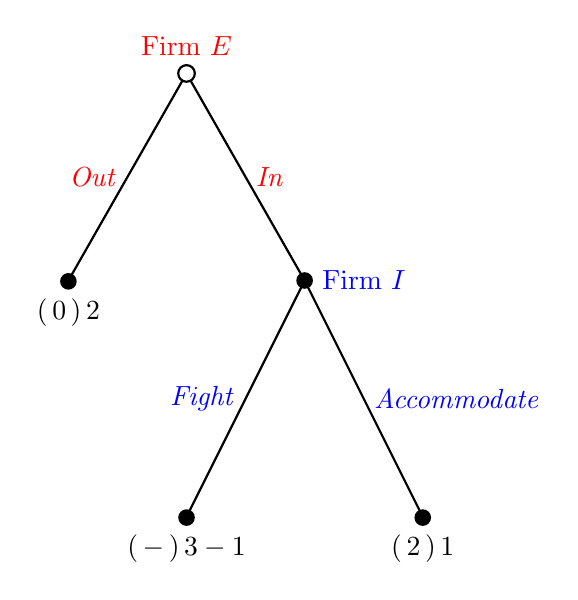
\begin{tikzpicture}[scale=1.5]
        \draw[thick] (0,0) -- (1,-1.753) node[pos=.5,right] {\color{red}\textit{In}};
        \draw[thick] (0,0) -- (-1,-1.753) node[pos=.5,left] {\color{red}\textit{Out}};
        \draw[thick] (1,-1.753) -- (2,-2-1.753) node[pos=.5,right] {\color{blue}\textit{Accommodate}};
        \draw[thick] (1,-1.753) -- (0,-2-1.753) node[pos=.5,left] {\color{blue}\textit{Fight}};
        \draw[fill=white, thick] (0,0) circle[radius=2pt];
        \node[above=0.1cm] at (0,0) {\color{red}Firm $E$};
        \fill (1,-1.753) circle (2pt) node[right=0.1cm] {\color{blue}Firm $I$};
        \fill (-1,-1.76) circle (2pt) node[below=0.1cm] {$\begin{pmatrix} 0 \\ 2 \end{pmatrix}$};
        \fill (0,-2-1.76) circle (2pt) node[below=0.1cm] {$\begin{pmatrix} -3 \\ -1 \end{pmatrix}$};
        \fill (2,-2-1.76) circle (2pt) node[below=0.1cm] {$\begin{pmatrix} 2 \\ 1 \end{pmatrix}$};
    \end{tikzpicture}
\end{figure}